\documentclass[../main/report.tex]{subfiles}
\begin{document}
\chapter{Discussion}

\section{Hardware components}
In this section we will discuss some of the physical design, alternative solutions and the practical solutions that arose during physical implementation.

\subsection*{USB data input}
In the initial design, a USB connector was introduced to receive data from a host PC. 
However, during the implementation phase it was discovered to be unnecessary.
We discovered that the software applications we wanted to run on the computer, could be included when programming the microcontroller with the JTAG.
This worked sufficiently for our needs. 
Since at the time we still had much else to do, implementing input by USB became a very low priority and in the end never happened.
This also applied to the serial backup as well.

\subsection*{VGA-port}
The PCB was designed with two VGA headers, one for the FPGA and one for the MCU. \todo{Maybe add picture showing the headers.}
Looking back, it was redundant to support two VGA ports.
An alternative solution is having one VGA port with exposed headers.
With exposed headers from the MCU and the FPGA as well, one could change which one the VGA port is connected to by jumpers like \ref{fig:vga-solution}.
By removing one of the VGA ports, the size of the PCB could have been reduced, or used for other components. 

\begin{figure}[H]
    \centering
    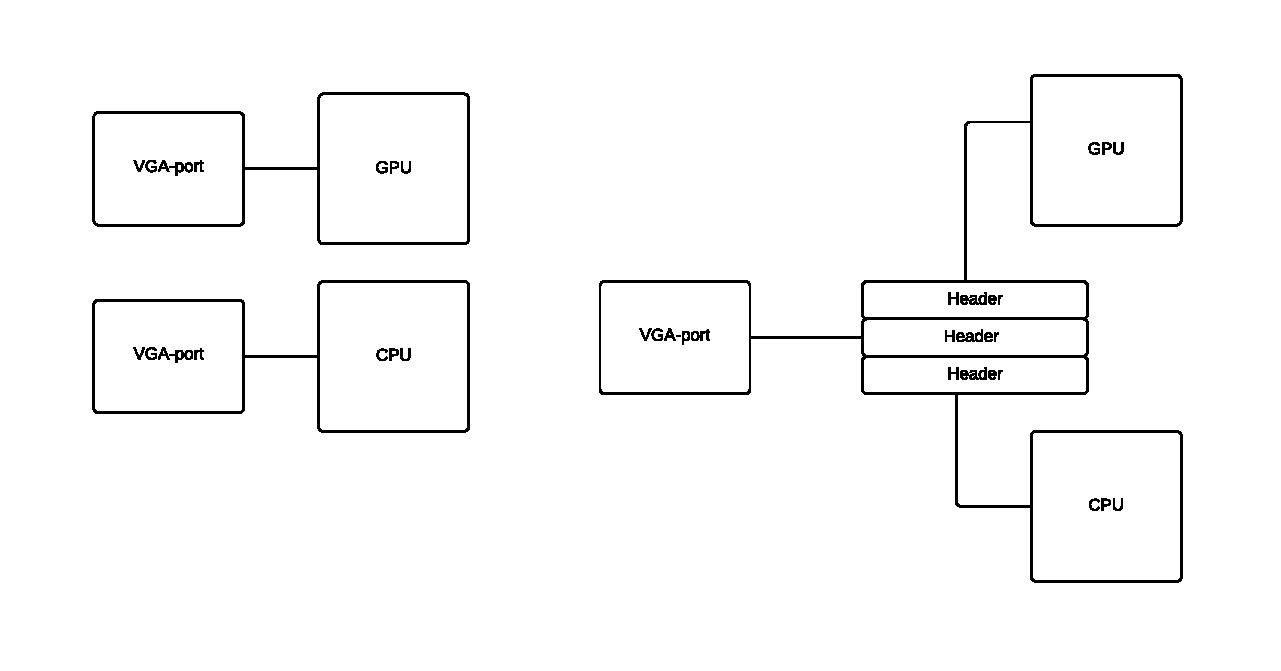
\includegraphics[width=\textwidth]{../discussion/assets/vga-solution.pdf}
    \label{fig:vga-solution}
    \caption{On the left: The current setup on our PCB. On the right: The alternative solution.}
\end{figure}

\subfile{../discussion/hacks.tex}

\subfile{../discussion/energy_efficiency.tex}

\section{"Jaktstart"}

Not everyone can start at the same time

\section{Redundancy design choices or w/e}
What did we end up needing?
What could we have used, that we didn't think of.

\section{Does the computer make sense?}
Is the design sane?
Were we idiots?
Have we seen the light?

\section{Can we even saturate the memory bus?}
Do you even SRAM?
Or is memory the big bottleneck

\section{SRAM bottleneck}
HDMI vs. the GPU?
Will the HDMI be fine with always being second in line?

\subfile{../discussion/budget.tex}

\end{document}
